\section{Introduction}

% \kwanghee{unify phone (phonetic) or phoneme (phonemic) across the full paper}
% \kwanghee{unify PR/UPR across the full paper}

\begin{figure}[t]
\centering
  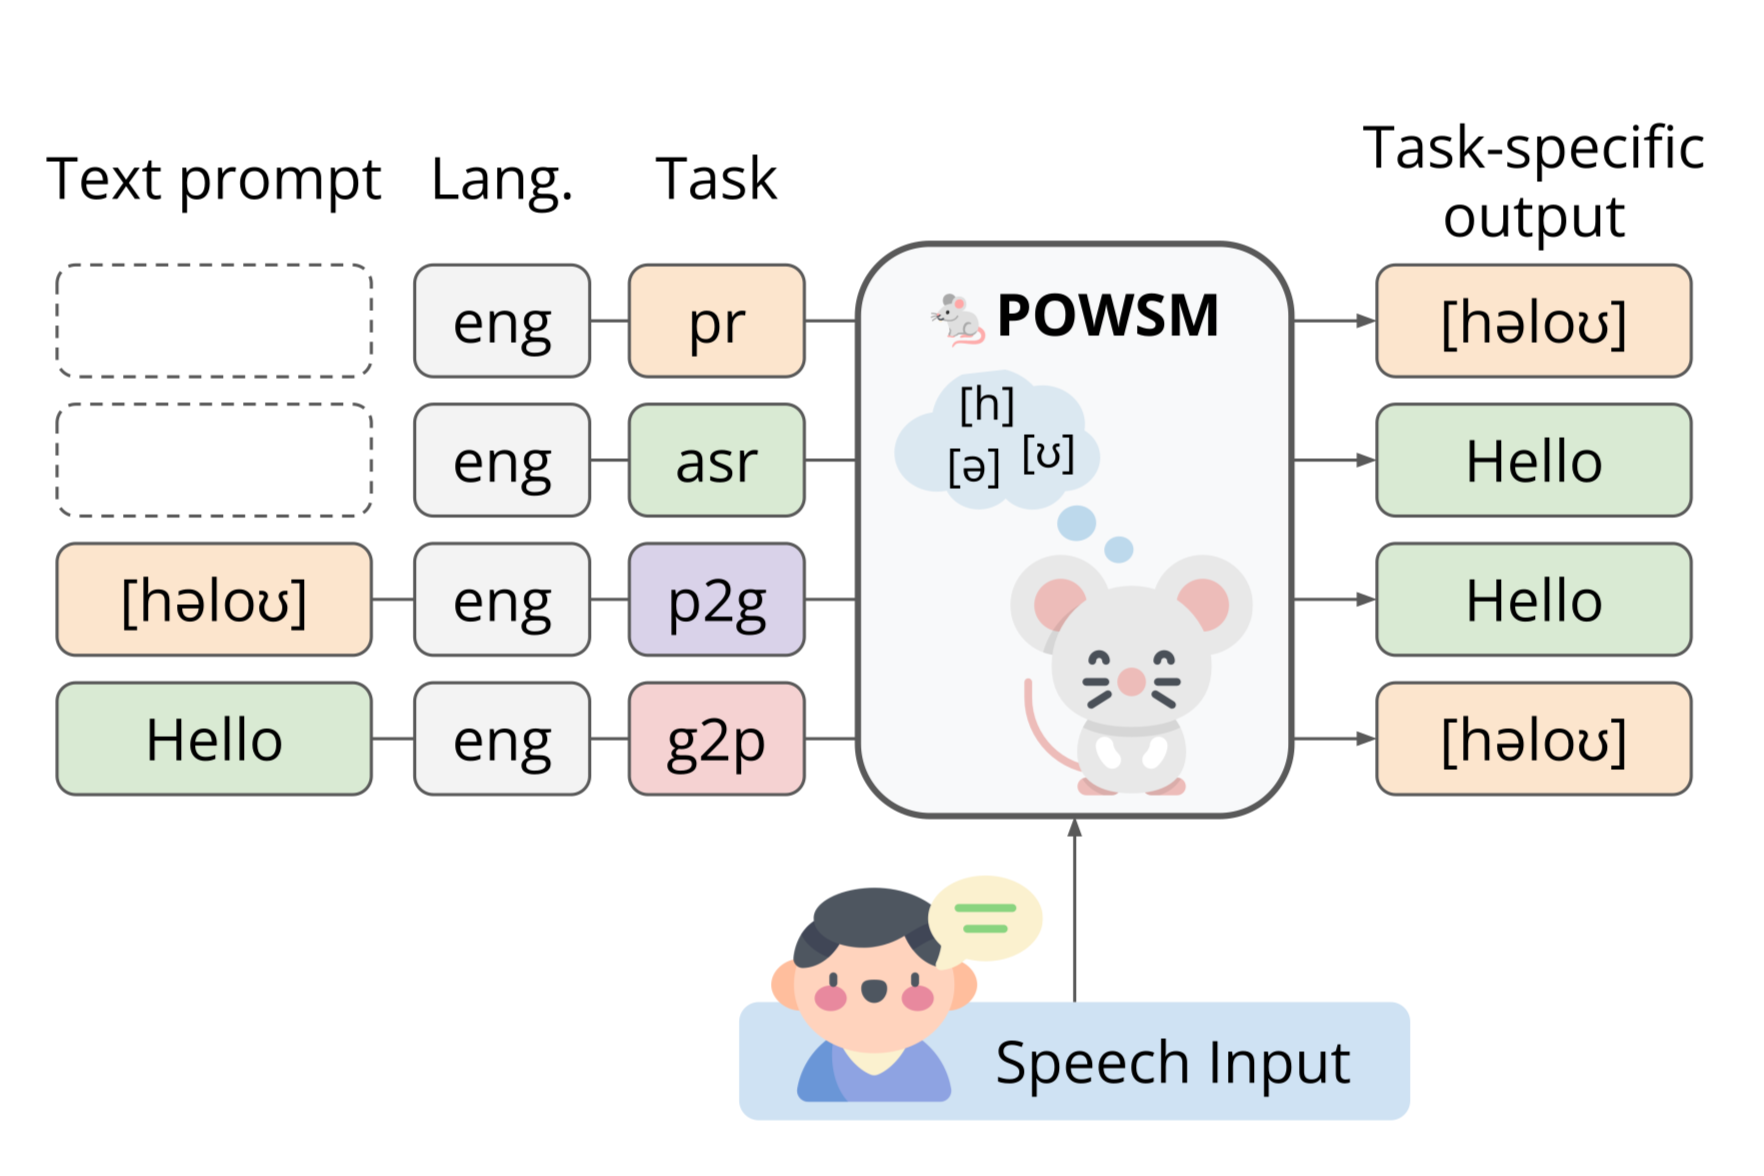
\includegraphics[width=\linewidth]{figures/main_figure.png}
  \caption{\POWSM is the first phonetic foundation model that can perform four phone-related tasks: Phone Recognition (PR), Automatic Speech Recognition (ASR), audio-guided grapheme-to-phoneme conversion (G2P), and audio-guided phoneme-to-grapheme conversion (P2G).
  }
  \label{fig:overview}
\end{figure}

% Fixed (3.2): \reviewer{Consider including a small qualitative example illustrating cross-task conversion (e.g., audio→phones→text) in the main text}
% Fixed: \reviewer{``phoneme-to-grapheme'' is occasionally written as ``P2G'' without consistent capitalization — ensure consistency.}

% Universal phone recognition (UPR) is the task of transcribing speech into phones, the smallest identifiable unit of sound in speech.
Phones are the smallest units of sound in speech. % distinctive -> phoneme
Unlike graphemes, phones are shared across languages and usually represented using the International Phonetic Alphabet (IPA) \citep{international1999handbook}, a unified transcription standard for all languages.
By providing a consistent representation of speech across languages, phone-level modeling allows fine-grained analysis and cross-lingual generalization, enabling tasks like atypical speech analysis (\textit{e.g.}, L2 speech \cite{li2016mispronunciation,inceoglu2023assessment} and pathological speech \cite{choi-etal-2025-leveraging, li2025towards}), endangered language documentation \cite{he-etal-2024-wav2gloss}, code-switched text-to-speech \cite{9054722}, and cross-lingual transfer in speech-to-text \cite{pratap2024scaling, magoshi25_interspeech}.

% pronunciation training \cite{kheir2025towards}, 
% child speech recognition \cite{dudy2018automatic, lin2024leveraging}, code-switched text-to-speech \cite{9054722}, and cross-lingual transfer in speech-to-text (S2T) \cite{pratap2024scaling, magoshi25_interspeech}.

Four key phone-related tasks underpin phonetic spoken language processing: automatic speech recognition (ASR), phone recognition (PR), grapheme-to-phoneme conversion (G2P), and phoneme-to-grapheme conversion (P2G).
\textit{ASR} learns implicit phonetic representations \cite{belinkov2017analyzing}, while \textit{PR} offers explicit phone-level supervision.
\textit{G2P} and \textit{P2G} bridge orthographic and phonetic spaces. 
Collectively, these tasks interact through shared phonetic representations, each addressing a different aspect of the relationship between audio, phones, phonemes, and graphemes.

Despite their conceptual similarity, these tasks have traditionally been developed in isolation, using task-specific architectures and datasets. 
Such systems are optimized for specific input-output mappings and cannot be easily extended to other phonetic tasks.
This fragmentation has hindered the development of general-purpose models for phonetic processing, necessitating a unified phonetic foundation model that can perform multiple phone-related tasks within a single, general framework for speech processing.

To bridge this gap, we propose \POWSM, a phonetic foundation model capable of performing four core phone-related tasks --- PR, ASR, audio-guided G2P, and audio-guided P2G --- within one unified architecture (\Cref{fig:overview}). 
To construct this framework, we reformulate standard ASR datasets \cite{zhu-etal-2025-zipa} into four task-specific formats, allowing the model to learn consistent mappings across audio, phoneme, and grapheme representations.
In addition, \POWSM adopts an attention-based encoder-decoder (AED) architecture, following the design of large-scale speech foundation models such as Whisper \citep{radford2023robust} and OWSM \citep{peng2023reproducing}.

% Fixed: \reviewer{consider breaking into two sentences for clarity.}
Empirically, \POWSM outperforms previous PR models on both in-domain data and out-of-domain languages and  achieves low-resource ASR performance comparable to web-scale multilingual foundation models. Moreover, it performs speech-grounded P2G and G2P across more than 70 languages.
\POWSM offers a new unified paradigm for phone-level modeling, paving the way for inclusive and globally accessible speech technologies that transcend language boundaries and resource disparities.

To summarize, our main contributions are: 
\begin{itemize}
    \item We release \POWSM, a large-scale foundation model that achieves state-of-the-art PR performance, and is capable of performing multiple fundamental phone-related tasks. Our model enables seamless conversion between speech, text (graphemes/orthography), and phones.
    \item We thoroughly analyze \POWSM to understand the interaction between multiple tasks, architecture components, and losses.
    \item We fully open-source all our data preparation and evaluation scripts, model checkpoint and code to foster open science.
\end{itemize}

% \POWSM is trained at scale and designed to solve all four major phone-related tasks by a single model.
% \POWSM follows the attention-based encoder decoder (AED) architecture, which is adopted by state-of-the-art foundation models such as Whisper \cite{radford2023robust} and OWSM \cite{peng2023reproducing}. 
% This allows the encoder to learn shared phonetic-acoustic representations, while the decoder can deploy these shared representations to perform specific tasks, \textit{i.e.}, PR, ASR, G2P, and P2G tasks, as illustrated in \autoref{figures/main_figure.png}
% \POWSM achieves better or competitive performance in PR than specialized models with roughly the same parameters \citep{xu22b_interspeech,zhu-etal-2025-zipa} yet is much more versatile in multi-tasking. % \jian{}

% We employ the AED architecture so that

% \POWSM improves PR performance by \shikhar{x\%} on \shikhar{A and B benchmarks}.
% In combination with training over a diverse set of languages, our multi-task approach to PR improves performance for unseen languages and socio-phonetic variation. 
%We also extend the unseen language sets to include Tusom \cite{mortensen2021tusom2021}, a low-resource variety, while expanding the socio-phonetic variation sets \kalvin{which part did we expand?}.



% Because manual phonemic transcription is highly labor-intensive \citep{he-etal-2024-wav2gloss}, \citet{zhu-etal-2025-zipa,xu22b_interspeech} have employed grapheme-to-phoneme (G2P) conversion to repurpose existing large-scale automatic speech recognition (ASR) datasets for phoneme recognition (PR).
% This naturally provides ground-truth text (grapheme) transcriptions for each phoneme transcription. % paired
% % \kalvin{data augmentation but not really data augmentation}
% Leveraging paired phoneme-text transcriptions, we are now able to train on three additional phone-related tasks using the same dataset: ASR, audio-guided G2P conversion, and audio-guided phoneme-to-grapheme (P2G) conversion. 
% \kalvin{define audio-guided}

% Advancing this multi-task agenda, we present \POWSM, a phonetic foundation model.


% Together, they provide complementary perspectives on the same phonetic continuum, forming the foundation for unified speech processing across languages. 

% As introduced in \Cref{fig:overview}, 

% Especially, phone recognition (PR), the task of transcribing speech into phones, facilitates these technologies by capturing details in speech that are missed by conventional grapheme-level S2T systems, \textit{e.g.}, automatic speech recognition (ASR), in a language-agnostic fashion.
% As shown in \autoref{fig:training}, UPR facilitates these tasks by capturing details in speech that are missed by conventional grapheme-level S2T systems (e.g. automatic speech recognition) in a language-agnostic fashion.
% Existing UPR systems demonstrate the promise of UPR for applications, but their current performance falls short of fully realizing their potential.
% \eunjung{I think the main limitation of ASR in this context should focus on its word-level / grapheme-level predictions. Since ASR outputs are constrained by a language model, it is expected that ASR to normalize atypical pronunciations with more probable words, thereby masking pronunciation deviations. In contrast, UPR aims to preserve the realized acoustic details of speech, directly reflecting pronunciation variations.
% For example, given the intended words snake [sneɪk], a conventional ASR system might output as sneak —substituting entire words. A phone recognizer, however, would produce [sneɪt], accurately revealing the speaker’s realized (mis)pronunciations.
% (I shared the example with Chin-Jou: Figure 1)}

% \kalvin{platform our use of graphemes first}
% While recent PR systems show strong potential, they overlook a simple but powerful insight: repurposing ASR transcripts can quadruple the training data.
% To scale the amount of data for UPR, we leverage an overlooked resource: the original ASR transcripts from which phoneme transcripts are derived. % I put this first b/c the focus is NOT on G2P, it's on our framework. david (and the writing center) suggest putting important ideas in the first sentence


% \kalvin{same speech, 4 diff tasks}
% We hypothesize that these additional tasks can enhance PR performance. 
% Specifically, we posit that the multi-task learning framework will expose the model to a broader range of linguistic information, enabling it to capture more higher-level linguistic structure such as morphology \citep{mohebbi-etal-2023-homophone}, syntax \citep{he2025layer,pasad2025speech}, and semantics \citep{pasad2025speech,ma-etal-2025-cross,shim2025languages}. % \kalvin{should we move this up to be the first sentence or is the current first sentence fine}
% mohebbi-etal-2023-homophone: morphosyntax (grammatical agreement - need to attend to syntactic cues)
% pasad2025speech: Syntactic content; CCA similarity between Whisper word segment representations and POS attributes
% phonology - syllable constituency in Whisper (Uncovering Syllable Constituents in the Self-Attention-Based Speech Representations of Whisper)
% Emergent morpho-phonological representations in self-supervised speech models - not whisper tho

% Kalvin's previous version
% Prior methods obtained phonemic transcriptions via grapheme-to-phoneme (G2P) conversion, but this approach introduces noise and removes fine-grained acoustic information---the very aspect that makes UPR valuable.
% Specifically, G2P enforces one global pronunciation for every orthographic type, even though there are multiple pronunciations due to context or variation \citep{zhu-etal-2025-zipa}. % \kalvin{another way to word this: ``the data enforces aone-to-one mapping between orthography and transcription''}
% For instance, ``crayon'' in American English can be pronounced as \ipa{/ˈkɹæn/}, \ipa{/ˈkɹej.ɔn/}, or \ipa{/ˈkɹej.ɒn/} \citep{vaux2003harvard} (among others).
% % Specifically, G2P normalizes phonetic variation by designating one pronunciation variant as the global representation \citep{zhu-etal-2025-zipa}, even within standard varieties of a language. For instance, ``crayon'' in American English can be pronounced as \ipa{/ˈkɹæn/}, \ipa{/ˈkɹej.ɔn/}, or \ipa{/ˈkɹej.ɒn/} \citep{vaux2003harvard} (among others).
% % One of the main obstacles is the lack of high-quality data. \drm{This is problematic because it foregrounds the data rather than foregrounding the solution. The problem is not that the data is of low quality, but that previous approaches have not been robust to low-quality data.}
% Despite these limitations, G2P is often applied to orthographic ASR (automatic speech recognition) datasets \cite{xu22b_interspeech, zhu-etal-2024-taste, zhu-etal-2025-zipa} because manual phoneme (and S2T) transcription is labor-intensive \citep{amith2021end,michaud2014towards} and requires linguistic expertise. 
% % Acquiring phoneme transcriptions for UPR remains difficult at a large scale, not only because of the labor involved in speech-to-text transcription in general  and due to the linguistic expertise required. % While this is not a major issue for most S2T tasks, it becomes critical for UPR, since G2P omits fine-grained acoustic information---the very aspect that makes UPR important---and simultaneously introduces noise. \drm{The last line is the important one; that claim should be moved to the beginning of the paragraph.}
% This limitation echoes how static word embeddings assign one global embedding per orthographic type (e.g. \textit{bank})---later solved with contextualized representations \cite{devlin2019bert}. % \textbf{Single Global Representation (SGR)} problem

% To address this problem, we posit that multi-task training that leverages the cleanliness of existing ASR transcripts (already in orthographic form) can regularize G2P-induced noise.
% \shinji{not sure if multi-task is a direct answer to SGR. Need further clarification}
% \eunjung{including ASR is good} \drm{acoustic signal to orthographic rep. ASR is more straight-forward, teaching the model about phonetic-knowledge in ..?} \kwanghee{not a direct answer to SGR, but whisper encoder, trained on ASR, behaves similar to SSL models, which means they are acoustic. The model implicitly split roles for enc and dec. Graphemes-signal are one-to-many, while phone-signal should be one-to-one (but it's not?). Training gradient would be cleaner if we include ASR.} \shikhar{collapsing targets if there's only PR. include P2G forces the model to capture model details, bc it have to convert it back to graphemes. 1: retain info from enc (what we want), 2: conserve phonotatics (what the model might be doing). }
%  % From a data-driven perspective, we hypothesize that G2P-induced noise limits the model’s ability to learn effectively from data, and that incorporating existing ASR transcripts may regularize this noise by associating pronunciation variants with canonical word forms. \drm{Phrase this positively: training on multiple tasks will have a regularizing function which will mitigate the effects of noisy data. Perhaps we need a name for data that is made noisy by having a single representation for every orthographically identical word. Note that representing text with static word embeddings produced the same problem. Context Agnostic Overgeneralization (CAO)?}
% Jointly training on UPR, ASR, G2P and P2G using the same speech data may ground phoneme representations in their acoustic realizations. % multiple S2T tasks using the same speech data: 
% % \drm{My intuition is that training the model to do G2P and P2G (and perhaps ASR) should force it to build more acoustically-grounded representations of phone (and perhaps more contextualized representations)}
% % Adding G2P and P2G in particular may learn more acoustically-grounded, contextualized phone representations.\kalvin{maybe add an example in the footnote b/c it's not obvious what is meant by this} %\drm{it’s going to learn, e.g., a single representation of \ipa{[θ]} that encompasses acoustic \ipa{[t]}, \ipa{[f]}, and \ipa{[s]}. }
% For instance, different English varieties realize \ipa{/θ/} as \ipa{[θ]}, \ipa{[t]}, \ipa{[f]}, and \ipa{[s]}. % socio-phonetic variation
% \kalvin{Only using G2P leads to \ipa{[θ]} as the global representation of \ipa{[θ]}, while using orthographies means all variants are tied to ... }
% \kalvin{now that i think about it, using only G2P will teach the model to map all phonetic variants/realizations to one phoneme (which may be bad but it's still contextualized) not sure how orthography will help, as it uses one representation for all word}
% \shikhar{
% % To address SGR, we posit that multi-task training combining UPR, ASR, G2P, and P2G can regularize G2P induced noise by anchoring phoneme learning to both acoustic and linguistic structure. 
% P2G enforces fine-grained acoustic grounding, while G2P introduces linguistic knowledge, jointly preventing overgeneralized representations (e.g., contextually specializing \ipa{[θ]} toward \ipa{[t]}, \ipa{[f]}, or \ipa{[s]}). <-- this is my attempt at handling shinji's comment succintly}
% \kalvin{how does P2G enforce fine-grained acoustic grounding?}
% \drm{general phonotatics patterns are shared across most languages, and we want enc-dec to handle diffeernt part. so we include aux tasks?}

% we're actually not directly addressing SGR. too complex
% engineering motivation: these data come from orthography. can cheaply use these transcriptions without much more effort.
% cite paper that shows that whisper has syntax/semantics
% framing: increasing the data (don't use data augmentation). using the same speech data in 4 diff ways is what makes us stand out.
% multi-tasking papers leverage similar tasks (multi-task learning helps learn intersection of diff tasks). this motivates shared encoder and decoder with task token
% RQ: can multi-tasking help PR?
% hyp: more ling knowledge can help PR

% \kalvin{we could also not talk about SGR but just focus on the regularization aspect? G2P loses phonetic precision (mapping all variants to one phone), which orthography mitigates with the coarseness of subword representations that capture more phonetic variants. it's good that G2P is more fine-grained than usual word-level/subword-level ASR, BUT noisy labels means it's honing in on the wrong details, which orthography fixes via regularization (bring it back to the coarse level)}
% \kwanghee{granularity of labels is not changing though. graphemes are coarser but we're not providing model with additional cue for more fine-grained details}
% \eunjung{this is more specific. we're not sure if the model is actually doing this, but we're sure that MTL is working}
% \kalvin{this is interesting interpretability follow-up work}

% \kalvin{unified modeling of speech, phones, and text is the only framing we can do given the results}

%%% Local Variables:
%%% mode: LaTeX
%%% TeX-engine: luatex
%%% TeX-master: "../main"
%%% End:


% \begin{figure}
%     \centering
%     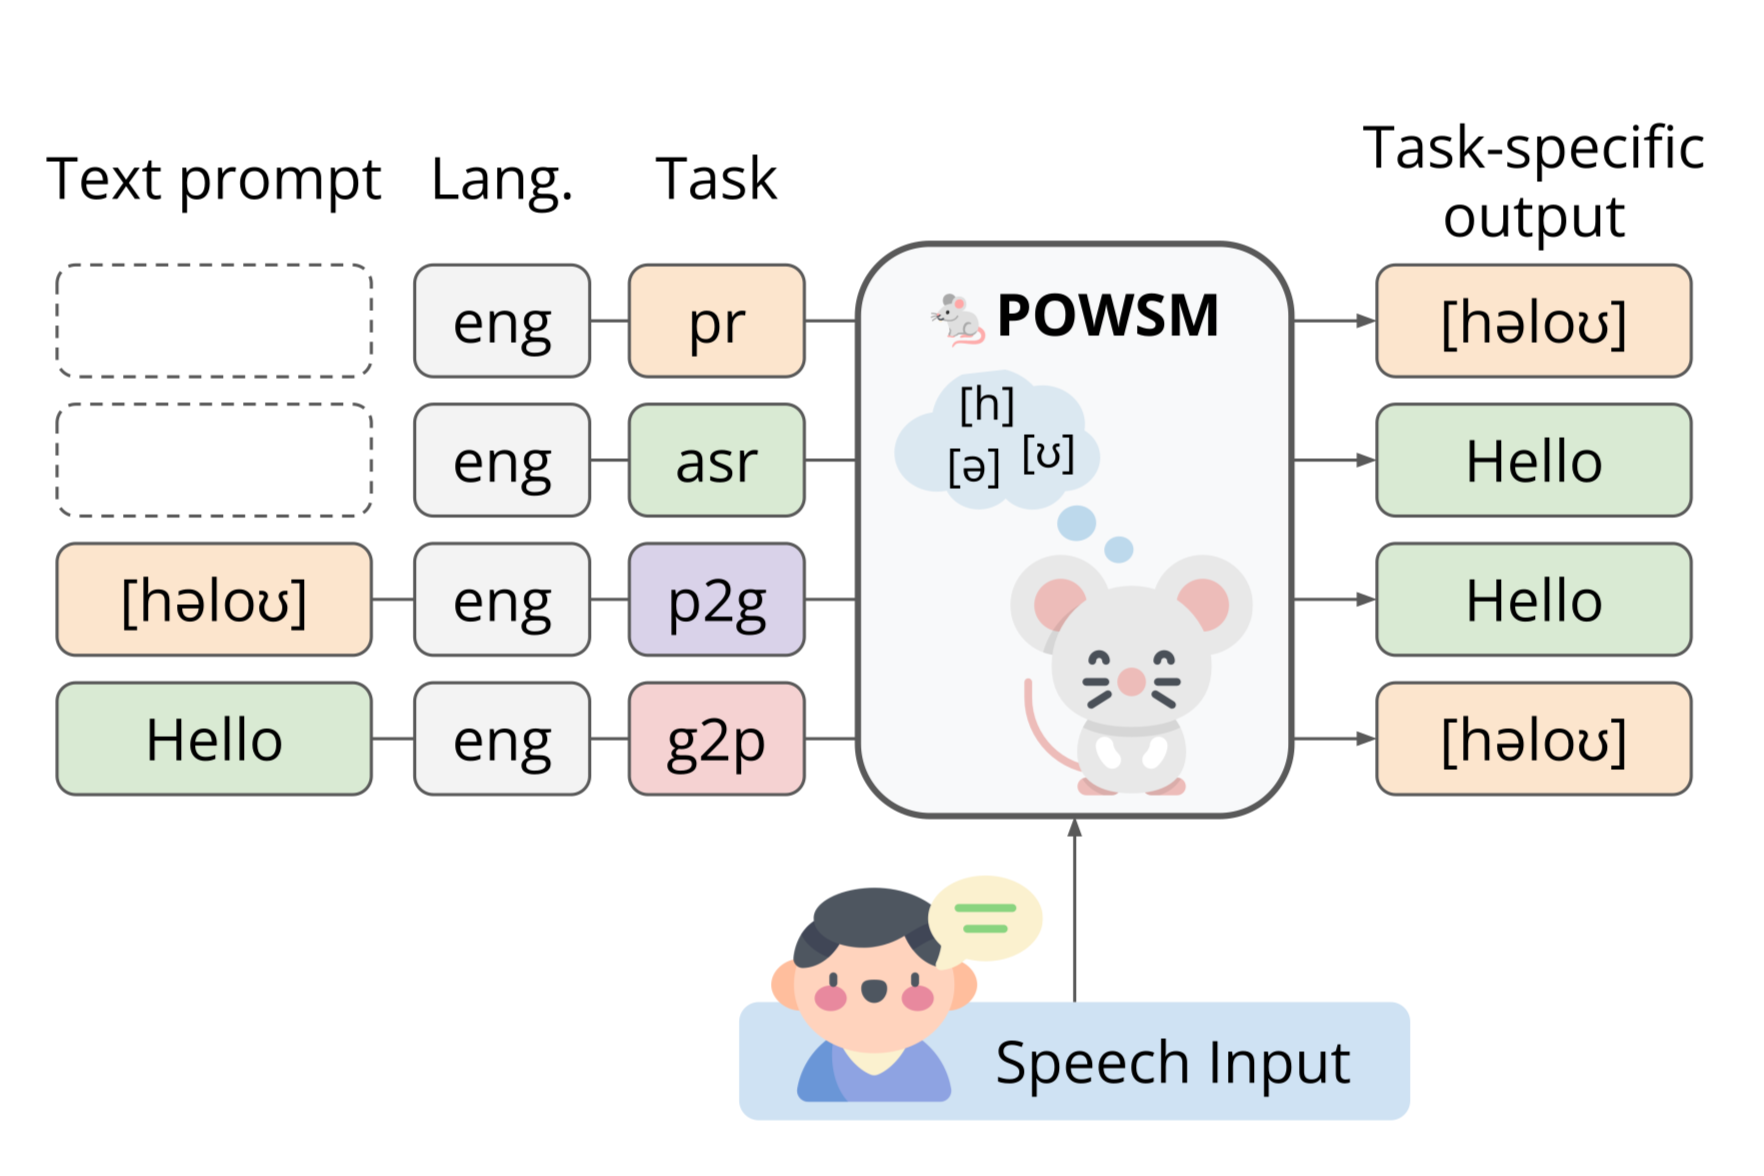
\includegraphics[width=0.95\textwidth]{figures/main_figure.png}
%     \caption{Multi-task setup of \POWSM, which encodes speech into representations guided by phone tokens, then predicts task-specific output.}
%     \label{fig:powsm}
% \end{figure}